%CTeX的report文档类   如果是article就用ctexart
\documentclass[a4paper,winfonts]{ctexrep}
% ------------------------------------------------------------------------------------------------------
%额外的数学符号支持
%\usepackage{amsthm}
%额外的注脚支持
\usepackage[stable]{footmisc}
%caption for environment
\usepackage{caption}
%页边距设置
\usepackage[top=0.8in,bottom=0.8in, left=0.8in, right=0.8in]{geometry}
%图片引用及格式支持
\usepackage{graphicx}
%长表格支持
\usepackage{longtable}
%more symbols
\usepackage{dingbat}
\usepackage{manfnt}
%超链接目录支持
\usepackage[CJKbookmarks=true,colorlinks,linkcolor=blue]{hyperref}    
%彩色支持、更多的色彩名称
\usepackage[usenames,dvipsnames]{color}
%代码高亮段支持
\usepackage{listings} %source code printing support
%subsubsubsection支持
\setcounter{secnumdepth}{5}
\renewcommand\theparagraph{\alph{paragraph}} \usepackage{lipsum}

%浅灰色(代码底色)
\definecolor{lightgray}{RGB}{230,230,230}
%常用emacs命令
%C-c C-q C-s(-e) Indentation
%C-c C-s new section
%C-c C-e new environment
%C-c C-c compile
%C-c C-v preview
\setmonofont{Courier New}
\lstset{ language={[ANSI]C},
         showspaces=false,
         showtabs=false,
         tabsize=4,
         frame=single,
         framerule=1pt,
         %numbers=left,
         %numberstyle=\small,
         basicstyle=\tt,
         directivestyle=\tt,
         identifierstyle=\tt,
         commentstyle=\tt,
         stringstyle=\tt,
         keywordstyle=\color{blue}\tt }
\usepackage{dirtree}

\begin{document}
% 设置章节标题格式
\CTEXsetup[format={\raggedright}]{chapter}
\CTEXsetup[format={\raggedright\Large\bfseries}]{section}
\CTEXsetup[format={\raggedright\large\bfseries}]{subsection}
\CTEXsetup[format={\raggedright\normalsize\bfseries}]{subsubsection}
% 设置代码引用格式
\lstset{language=C, numbers=left, basicstyle=\small,
  keywordstyle=\color{blue}, commentstyle=\color{PineGreen},
  stringstyle=\color{red}, frame=shadowbox, breaklines=true,
  backgroundcolor=\color{lightgray}, extendedchars=true
}
%
%封面
\newcommand{\HRule}{\rule{\linewidth}{0.5mm}}
\begin{titlepage}
	\begin{center}
		\phantom{placeholder}
		\vspace{6cm}
		\textsc{\LARGE Unicore32-MiniC }{\LARGE 实习报告}\\[2cm]
		\HRule\\[5cm]
		\begin{minipage}{0.4\textwidth}
			\begin{center} \large
				\emph{作者:}\\
				彭焯\\
				华连盛\\ 
				王衎\\
				李春奇\\ 
			\end{center}
		\end{minipage}
		\begin{minipage}{0.4\textwidth}
			\begin{center} \large
				\emph{ID} \\
				00848xxx\\
				00848xxx\\
				00848xxx\\
				00848xxx\\
			\end{center}
		\end{minipage}

		\vfill

		% Bottom of the page
		{\large \today}

	\end{center}

\end{titlepage}

\tableofcontents
\chapter*{简介}
\section*{如何阅读本文档}
下面给出了本文档的结构,单击目录树上的节点便可以查看文档的相关部分。
%\dirtree{%
%.1 intro.
%.2 a. 
%.1 b. 
%.2 c. 
%.3 d. 
%}
\label{pagetree}
\DTsetlength{1em}{5em}{0.3em}{1pt}{1.6pt}
\renewcommand*\DTstyle{\ttfamily}
\dirtree{%
.1 \hyperref[pagetree]{Unicore-MiniC 编译器}.
.2 \hyperref[flexbison]{词法、语法分析}.
.3 \hyperref[flex]{词法分析, flex}.
.3 \hyperref[bison]{语法分析, bison}.
.3 \hyperref[syntexerror]{语法错误检查}.
.3 \hyperref[pitfallc1]{谬误与陷阱}.
.2 \hyperref[intermidiate]{中间表示}.
.3 \hyperref[AST]{抽象语法树AST}.
.4 \hyperref[genAST]{生成}.
.4 \hyperref[symtbl]{符号表}.
.5 \hyperref[declchk]{声明错误检查}.
.4 \hyperref[typeveri]{类型检查}.
.3 \hyperref[triple]{三元式表示}.
.4 \hyperref[tripleinst]{三元式指令列表}.
.4 \hyperref[triplestruct]{三元式结构}.
.4 \hyperref[ASTtotriple]{将AST转化为三元式}.
.4 \hyperref[basicblock]{生成基本块}.
.3 \hyperref[indepopt]{机器无关优化}.
.4 活跃变量分析.
.4 数据流分析.
.4 (TODO).
.3 谬误与陷阱.
.2 目标代码.
.3 编译器-目标机器接口, 二进制规范.
.3 寄存器分配.
.3 运行时内存分配,栈帧,全局区,立即数.
.3 机器相关优化.
.4 特殊指令的使用.
.4 指令调度.
.3 谬误与陷阱.
.2 编译-体系联合实验.
.3 系统调用.
}
\section*{本文档包括的内容}
本文档的目标\emph{并不是}用于展示MiniC冗杂的代码,而是提供一个概括的全局视角来了解这个实习项目。\\
文档涵盖了如下的几个方面:
\begin{itemize}
	\item Unicore-MiniC编译器(以下在没有歧义的情况下简称之为MiniC)的总体设计方案
	\item MiniC的各个单元的设计方案,包括主要的数据结构和重要的算法
	\item MiniC各个单元之间的协同关系
	\item 为相关代码的阅读提供的指引
	\item 在开发过程中遇到的困难,遭遇的陷阱和付出的代价\footnote{参见某些章中的“谬误与陷阱”一节}
\end{itemize}
\section*{\textsc{MiniC In a Nutshell}}
\subsection*{项目目标}
\begin{itemize}
	\item 输入MiniC源代码,输出Unicore32汇编代码
	\item 利用Unicore32二进制工具链中的链结器链接后的程序能在 Unicore32 实体机器上运行
	\item 链接后的程序能够在同时设计的 Unicore32 模拟器上运行
	\item 通过对模拟器相关参数、指令系统的修改,考察编译-ISA 对性能的综合影响
\end{itemize}
整个项目将全部以C语言实现,用\verb|gcc|进行编译;以\verb|GNU/Linux, i386|为运行平台。使用\verb|svn|进行版本控制。项目主页:\href{http://code.google.com/p/minic}{code.google.com/p/minic}
\subsection*{项目结构}
下面是一个MiniC编译器的总体结构图:
\begin{center}
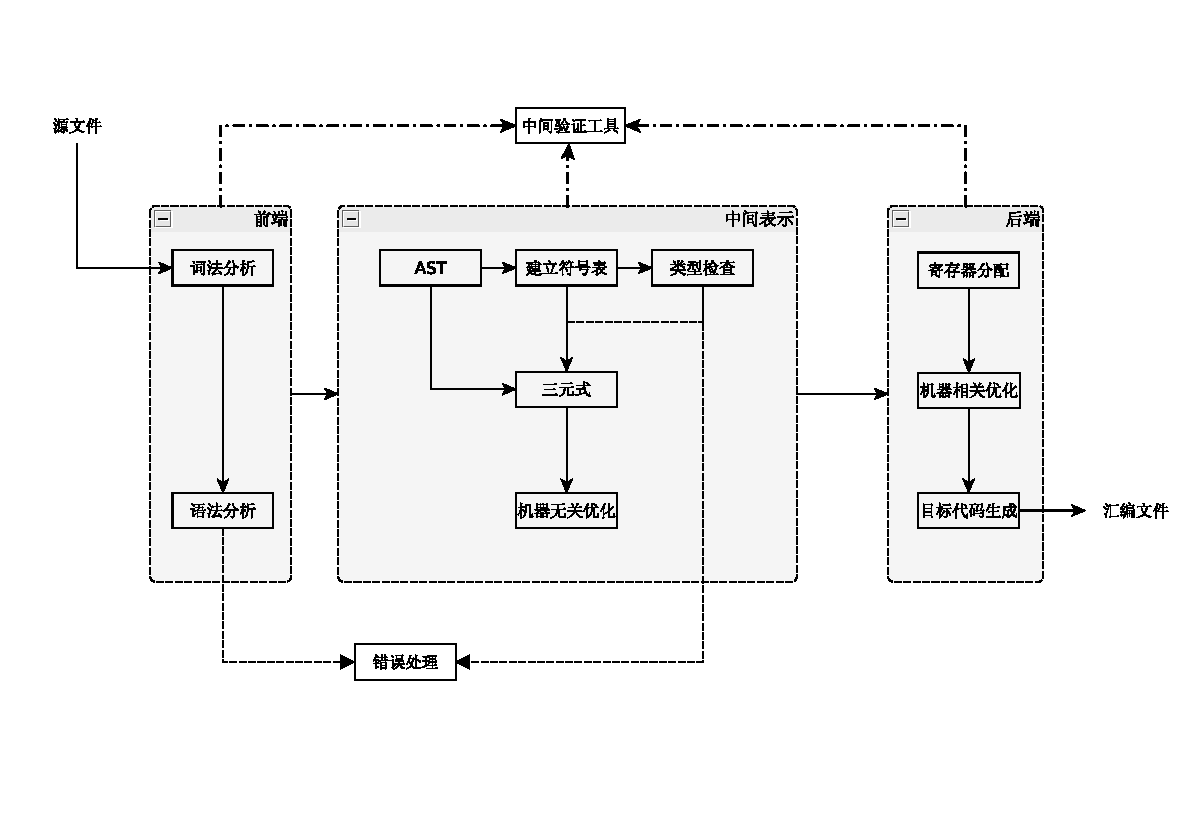
\includegraphics[scale=0.7]{main_structure.eps}
\end{center}
总体上看,MiniC由三大模块构成:
\begin{enumerate}
\item 前端:接收输入文件,结合文法,负责语法、词法分析;将源文件的结构和内容信息提取到抽象语法树(AST)上
\item 中间表示:共有两层:AST和三元式;语义分析在AST上完成后,将AST变换为三元式;机器无关优化在三元式表示上进行。
\item 后端:目标机器代码(汇编代码)生成;结合目标机器二进制规范和ISA,生成目标代码;机器相关优化在目标代码上进行。
\end{enumerate}
与此同时,还有错误处理模块,用于在源文件有误时产生出错提示;中间验证工具集,用于检查工程进展的每一个步骤的正确性。

在下面的章节中,我们将一一介绍以上模块,并且还将在最后一章展示MiniC编译器是如何与体系实习的模拟器项目配合,进行一系列编译-体系相关的实验和评测。

\section*{致谢}
\begin{itemize}
\item 感谢刘先华老师对我们小组的指导。他总能及时、耐心地解答我们的问题,与此同时又鼓励我们积极思考和大胆尝试,使我们从这个实习项目中收获了知识和快乐。

\item 感谢刘锋老师在工程进展和规划、模拟器-编译器结合方面提供的帮助。

\item 感谢与我们一同选择MiniC项目的另外两个小组的成员,你们的帮助和启发使我们受益匪浅。

\item 当然,最需要感谢的是这个项目本身:我们通过它同时体验了CPU设计人员、模拟器设计人员、甚至是(一部分)操作系统设计人员在设计一个大型的、可靠的系统时所面临的挑战,以及克服这些挑战后所获得的成就感。
\end{itemize}

下面,我们将从头开始,介绍\textsc{Unicore-MiniC}编译器。


\chapter{词法、语法分析}
\label{flexbison}
\section{词法分析, flex}
\label{flex}
词法分析的目的是将输入的源文件中的符号识别为语法分析器能够接受的tokens。其基本原理是利用正则表达式pattern来匹配、分割源文件中的符号。同时,词法分析还需要识别并保存一些名字和常量,比如函数名、变量名和字符串常量。

MiniC的词法规则同标准C的对应规则基本相同:
\begin{enumerate}
	\item 标识符必须以下划线或大小写字母开头,由下划线、大小写字母和数字组成
	\item 字符常量需要放在单引号\verb|''|中,字符串常量需要放在双引号\verb|""|中
	\item 有如下保留字不能当作标识符:\verb|extern|, \verb|register|, \verb|void|, \verb|int|, \verb|char|, \verb|if|, \verb|else|, \verb|for|, \verb|while|, \verb|return|
	\item 特殊符号包括:\verb#{}, (), [], +, -, *, !, &, =, |, >, <#
\end{enumerate}
由于语法分析器bison实际上不能获得\hyperref[ASTnode]{AST叶节点}上的信息,因此生成AST叶节点的工作交由flex完成。\\
\noindent
{\it \anchor flex源文件请参阅:\verb|minic.l|}
\section{语法分析, bison}
\label{bison}
语法分析的目的是根据语言的BNF范式,将词法分析器提交的token流进行规约,在规约的同时应用一些语法规则。语法分析的结果有两个:
\begin{enumerate}
	\item 将\emph{语法正确}的源文件转换为语法规则所要求的中间形式,这一中间形式不在具有语言的语法特性,或
	\item 发现语法错误,如果错误能够暂时恢复,就继续语法分析,在完成后提示错误信息;否则,直接停止语法分析,报告错误。
\end{enumerate}
MiniC项目利用bison辅助进行语法分析,分析完成后,将建立一棵AST。

在介绍对bison的利用前,由于我们的项目修改了给定的MiniC文法,所以首先要对修改后的文法进行说明。
\subsection{MiniC文法}
{\noindent \it \anchor 本项目的全部BNF范式请参阅:\verb|BNF|}\\
我们对原MiniC文法的改动主要在其表达式文法部分。

\section{语法错误检查}

\chapter{中间表示}
\label{intermidiate}
编译器的目的是将源文件“翻译”成目标机器的汇编文件。为了减小在翻译过程中所面对的源语言和目标汇编语言之间的复杂程度差距,编译器一般会将源文件变换成若干种中间表示,这些中间表示同目标汇编语言的相似程度逐渐增大。同时,在一些中间表示上,编译器能够相对容易地进行语义检查;在另一些些中间表示上,编译器还能利用相对简单、与源语言和目标汇编语言分别隔离的中间表示来进行机器无关优化。

MiniC采用了两重中间表示:抽象语法树(Abstract Syntax Tree)和三元式。语义检查在前者上完成,机器无关优化在后者上完成。下面将介绍这两种中间表示的生成以及在其上所做的相关工作。

\section{抽象语法树AST}
\label{AST}
AST是MiniC采用的第一重中间表示,它由在词法/语法分析阶段生成。由于我们在AST上完成了符号表的生成和类型检查,因此这两部分也在本章介绍。
\subsection{生成}
\label{genAST}
AST的结构是根据上下文无关文法的产生式定义的:一个终结符节点是一棵AST;一棵以产生式左部非终结符为根的AST的子节点按从左到右顺序分别是其右部分法符号所产生的AST。

比如有如下产生式:
\begin{displaymath}
	A:=aBcD
\end{displaymath}
其中大写字母代表非终结符,小写字母代表终结符,那么以非终结符A为根的AST就是如下形式:
\dirtree{%
.1 A.
.2 a.
.2 以非终结符B为根的AST.
.2 c.
.2 以非终结符D为根的AST.
}
注意到AST的定义实际上也给出了其产生方法:只要在做LR分析时,随着规约的进行,将子树与根进行连接即可。

在实现时,AST的叶节点在词法分析时生成,内部节点在语法分析时在不同的产生式的语法规则指导下生成,并在规约时连接到其父节点上。

下面给出一个MiniC的AST节点所包含的内容:
\label{ASTnode}
\begin{lstlisting}
typedef struct AST_NODE{
  	int nodeType;//节点类型,即节点代表了哪个文法符号
  	int nodeLevel;//节点深度
	union node_content content; //节点包含的内容,只有叶子节点才不为空,在词法分析时添加
  	AST_NODE * father;//父节点
  	AST_NODE * leftChild;//最左子节点
  	AST_NODE * rightSibling;//右兄弟节点

	struct symtbl_hdr* symtbl;//文法符号所在范围的符号表
	AST_NODE* double_list;
}AST_NODE;
\end{lstlisting}
{\it \anchor 有关节点类型的详细定义,请参阅:\verb|AST.h|}\\
{\it \anchor 有关建立AST树的相应过程,请参阅:\verb|AST_operation.c|, \verb|minic.y|}\\
\subsection{生成的语法树示例}
我们利用\verb|dot|生成了下面代码的AST:
\begin{lstlisting}
int main()
{
	int i;
	i = i + 1;
}

\end{lstlisting}

\begin{center}
	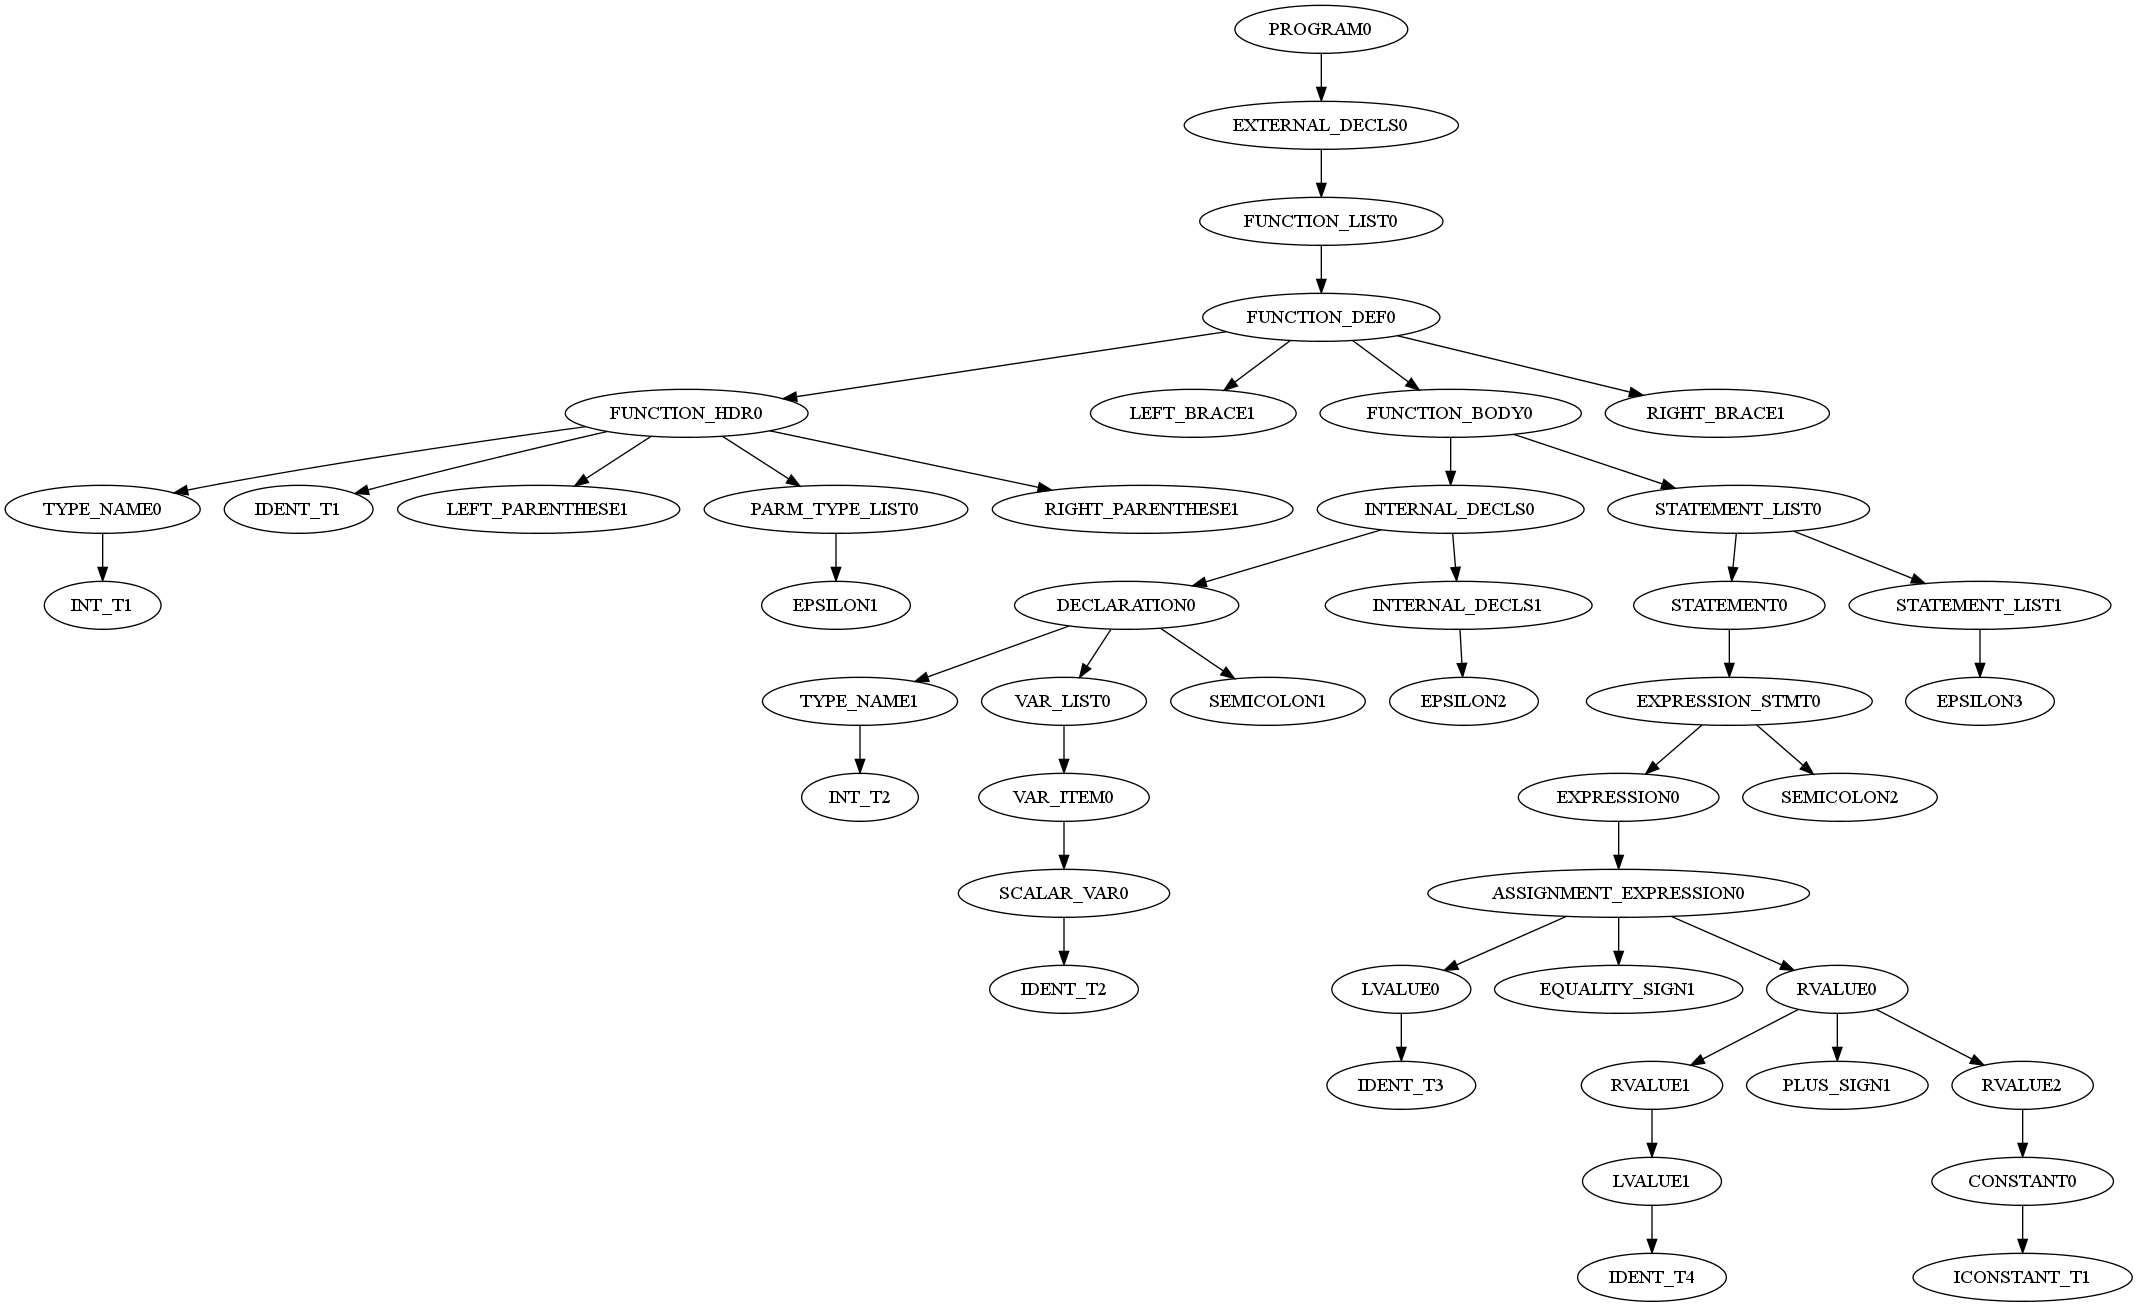
\includegraphics[scale=0.2]{grammer_tree.png}
	\captionof{figure}{AST示例}
	\label{fig:grammertree}
\end{center}
{\it \manerrarrow MiniC的验证工具中提供了两种方式查看输入源文件的语法树:\verb|dot|和ASCII ART,请参阅MiniC使用手册}\\
\subsection{AST的通用周游模板}
\label{ASTtravesal}
由于建立符号表、类型检查以及将AST变换成三元式都涉及到在AST上做深度游先周游,所以我们设计了一个通用的周游函数\verb|tree_traversal|,该函数接受两个参数:AST的根节点指针以及返回值为\verb|int|,参数为AST节点指针的函数指针的数组。由于我们将所有的节点类型都定义成了不同的整数,因此只需要为不同的周游阶段构造不同的函数指针数组,在\verb|tree_traversal|中周游到某个节点时以节点类型为数组下标定位到对这个节点进行操作的函数并调用,就能够用同一个深度游先周游函数完成不同的周游功能。\\
{\it \anchor 有关深度优先周游模板的代码,请参阅:\verb|symtbl_operation.h|}\\

\subsection{符号表}
\label{symtbl}
符号表对于一个编译程序而言是最为重要的一个部分,从它创建以后开始的每一个步骤中,“标识符”(函数名、变量名)的出现,就意味着要在符号表中找到对应的表项,提取要使用的信息。

\paragraph*{符号表的结构}
符号表的层次结构需要根据语言的特性来决定。例如在MiniC中,由于存在着全局变量、函数声明、语句块等特点,因此符号表需要组织成树状结构。

符号表的具体底层数据结构可以有很多种选择,常见的有哈希表、链表和线性表,在MiniC中,由于考虑到输入源文件的规模都较小,所以采用可扩张的线性表来实现\footnote{这种线性表在空间不足时会另外申请一块两倍的空间并拷贝自己}。在这种实现下,插入一个表项的均摊开销是$O(1)$,检索一个表项的开销是$O(n)$,$n$为表项总数目。


MiniC的符号表结构如下:
\begin{enumerate}
\item 每个作用域(函数、复合语句)一张符号表:
\begin{lstlisting}
struct symtbl_hdr
{
	symtbl_hdr* parent_tbl; //父表
	symtbl_hdr* leftChild_tbl; //最左子表
	symtbl_hdr* rightSibling_tbl;	//右兄弟子表

	//ret_type, ret_star, para_num, func are useful only for function's symtbl
	char* func_name; //函数名,若该表属于复合语句则该项为空
	int ret_type; //函数返回值基类型
	int ret_star; //函数返回值是否为指针类型
	int para_num; //该函数的参数个数
	int func_def; //该函数是否有定义
	int item_num; //符号表表项数目
	int maxSize; //全部表项占用的内存大小,字节
	symtbl_item* item; //表项列表
}
\end{lstlisting}
\item 每张符号表都有一个表项列表:
\begin{lstlisting}
struct symtbl_item
{
	int isGlobal; //是否为全局变量
	int type; //表项的基类型
	int star_num; //表项是否为指针
	int writable; //表项是否为只读类型
	char* name; //符号名 
	int size; //数组大小,非数组为0
	int func_off; //
	int offset; //在内存分配中的偏移
};

\end{lstlisting}
\end{enumerate}
注意到在一个函数的符号表中,函数的参数和它的局部变量是存放在一起的,这种将参数和局部变量视作同类的安排能够为以后的内存分配、寄存器分配等提供一些方便。



\paragraph*{在AST上生成符号表}
如前所述,AST上包含了源文件中所有的信息,因此只需要扫描AST的某些子树,提取符号名称、类型、作用域等信息,就可以生成符号表。

具体的做法是:先序深度优先周游AST,找到作用域入口(\verb|FUNCTION_DEF|和\verb|COMPOUND_STMT|)并将当前作用于压入作用域栈,然后在该作用域节点下寻找类型为\verb|EXTERNAL_DECLS|和\verb|INTERNAL_DECLS|的节点,分情况处理该节点的函数和变量的声明,将名称和类型(包括函数的返回类型,参数、参数类型)加入符号表,作用域从作用域栈顶取得。在作用域出口(周游函数返回时)弹出作用域栈顶。\\
{\it \anchor 有关符号表生成的相关代码,请参阅:\verb|gen_symtbl.h|}\\

\paragraph*{在符号表上查询符号}
由于符号表是树状组织,因此查询时要从给定的一张符号表开始,在表中查找,如果未找到符号,就在当前表的父表中查找,直到找到该符号或者在最高级的\verb|Global Scope|也没有找到返回空。
\\
{\it \anchor 有关符号表查询的代码,请参阅:\verb|symtbl_operation.h|}\\
\paragraph*{符号表生成与语义检查}
\label{declchk}
在符号表生成的过程中,实际上还要进行一项语义检查:同一作用域的多重定义问题。即在向当前符号表中添加符号时,如果该符号已经出现在了当前表中,就要报告错误,停止建立符号表。

\subsection{符号表示例}
下图展示了以下代码的符号表:
\begin{lstlisting}
int i,j;
void f(int k)
{
	int i,j;
}
int main()
{
	int i,j;
	{int k;}
}
\end{lstlisting}
\begin{center}
	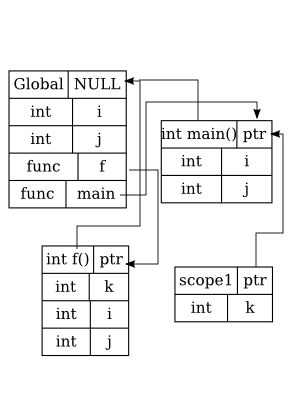
\includegraphics[scale=0.6]{symtbl.png}
	\captionof{figure}{符号表示例}
\end{center}
{\it \manerrarrow MiniC的验证工具中提供了查看源文件生成的符号表的方法:请参阅MiniC使用手册}\\
\subsection{类型检查}
\label{typeveri}
类型检查是语义检查的一部分,这一步骤的主要目的是排除所有符合语法但不符合运算规则、函数调用规则的语句。类型检查的对象是表达式语句,这包括:
\begin{itemize}
	\item 检查一元、二元运算符作用的对象;报告类型无效的运算对象
	\item 检查传入函数的实参类型和函数的参数表对应形参的类型是否兼容;报告兼容性警告或者错误
	\item 检查赋值语句两边类型是否是赋值兼容的(包括检查函数返回值);报告兼容性警告或者错误
\end{itemize}
类型检查一旦完成,表明这份源代码已经能够且必须通过后续的变换,直到生成目标代码。
\paragraph*{类型检查的规则} 下面的表格给出了MiniC类型检查的所有规则以及应对方法。
%TODO: 类型检查规则表 from 毛哥
\paragraph*{在AST上做类型检查}
类似于生成符号表,类型检查同样要对AST进行深度优先周游,在发现\verb|STATMENT|类型的节点时开始按照不同的语句类型以及语句中不同的元素类型开始进行类型检查。


\section{三元式}
\label{triple}
三元式是MiniC的第二重中间表示。同MiniC源文件中复杂的语句和操作相比,三元式相对简单、只有少数指令并且更接近目标代码表示。

MiniC中,一条三元式可以表示为如下形式:
\begin{itemize}
\item A: 一般的运算指令:\verb|(i): op arg1, arg2|, \verb|arg|可以是\verb|(j)|也可以是标识符或立即数;\verb|arg2|若无效则为单元操作
\item B: 条件跳转指令:\verb|(i): if arg goto (j)|,\verb|arg|可以是\verb|(j)|也可以是标识符或立即数
\item C: 无条件跳转指令:\verb|(i): goto (j)|
\item D: 传参指令:\verb|(i): param arg|,\verb|arg|可以是\verb|(j)|也可以是标识符或立即数;出现在调用指令前
\item E: 调用指令:\verb|(i): call (j)|
\item F: 作用域指令:\verb|(i): enter|, \verb|(i): leave|用于指示作用域的变化
\item G: 布尔专用指令:\verb|(i): setrb|, \verb|(i): getrb|用于组合布尔表达式的翻译,后面会有详细叙述
\end{itemize}
\subsection{三元式的结构}
\label{triplestruct}
考虑到后续在三元式上的操作,三元式并不以上述的字符串的形式储存,以结构的形式存在一个可扩张的线性表中(类似于符号表的实现)。下面给出表项的结构:
\begin{lstlisting}
typedef struct triple
{
	enum operator op;
	union arg arg1;
	union arg arg2;
	int result_type; //运算结果的类型
	int arg1_type; //参量的类型
	int arg2_type; 
	symtbl_hdr* symtbl; //本条三元式所属范围的符号表
	struct basic_block *block; //本条三元式所属的基本块
	int arg1_uni; //“联合查询表”中第一个参数的编号
	int arg2_uni; //“联合查询表”中第二个参数的编号
	int tmp_uni; //“联合查询表”中三元式标号(临时变量)的编号
	int label; //本条三元式的标号(仅当本条三元式是跳转语句的目标时有效)
}triple;
\end{lstlisting}
有关“联合查询表”的作用,参见“机器无关优化”一节的\hyperref[jointtable]{“基础数据结构”}。
\subsection{三元式指令列表}
\label{tripleinst}
下面的表格给出了MiniC的三元式中所有的\verb|op|以及对应的功能和三元式类型(每种类型的具体解释见本节起始处的说明):
\begin{center}
\begin{minipage}{0.48\textwidth}
\begin{flushleft}
	\begin{tabular}{|l|l|l|}
	\hline
		\verb|op| & 类型 & 功能 \\
	\hline
		\verb|if| & B & 条件成立就跳转 \\
	\hline
		\verb|if_not| & B & 条件不成立就跳转 \\
	\hline
		\verb|goto| & C & 无条件跳转\\
	\hline 
		\verb|negative| & A & 取相反数\\
	\hline
		\verb|not| & A & 取布尔非\\
	\hline
		\verb|address| & A & 取地址\\
	\hline
		\verb|star| & A & 取地址处存放的数据\\
	\hline
		\verb|positive| & A & 返回操作数本身\\
	\hline
		\verb|assign| & A & 值赋给\verb|arg1|\\
	\hline
		\verb|star_assign| & A & 赋值给地址\\
	\hline 
		\verb|add| & A & 加法\\
	\hline 
		\verb|minus| & A & 减法\\
	\hline
		\verb|multiply| & A & 乘法\\
	\hline 
		\verb|char_to_int| & A & 类型转换\\
	\hline
		\verb|equal| & A & 判断相等\\
	\hline
		\verb|less| & A & 判断是否小于\\
	\hline 
		\verb|larger| & A & 判断是否大于\\
	\hline
		\verb|eqlarger| & A & 判断是否大于等于\\
	\hline
	\end{tabular} 
\end{flushleft}
\end{minipage}
\begin{minipage}{0.48\textwidth}
\begin{flushright}
\begin{tabular}{|l|l|l|}
	\hline
		\verb|op| & 类型 & 功能 \\
	\hline
		\verb|eqless| & A & 判读是否小于等于\\
	\hline 
		\verb|noteq| & A & 判读是否不等于\\
	\hline 
		\verb|or| & A & 布尔或\\
	\hline 
		\verb|and| & A & 布尔与\\
	\hline 
		\verb|setrb| & G & 将\verb|rb|置为\verb|arg|的值\\
	\hline 
		\verb|getrb| & G & 获取\verb|rb|的值\\
	\hline 
		\verb|call| & E & 调用函数\\
	\hline 
		\verb|param| & D & 传参\\
	\hline 
		\verb|enterF| & F & 进入函数\\
	\hline 
		\verb|enterS| & F & 进入复合语句\\
	\hline 
		\verb|leaveF| & F & 离开函数\\
	\hline 
		\verb|leaveS| & F & 离开复合语句\\
	\hline 
		\verb|return| & A & 返回\\
	\hline
		\verb|adds| & A & 左移两位后加\\
	\hline
		\verb|minuss| & A & 左移两位后减\\
	\hline 
		\verb|r_shift| & A & 右移两位\\
	\hline 
		\verb|c_str| & A & 表示一个字符串\\
	\hline
		\verb|Imm| & A & 表示一个大于511的立即数\\
	\hline
	\end{tabular}
\end{flushright}
\end{minipage}
	\captionof{table}{MiniC三元式\lstinline|op|定义}
\end{center}
\subsection{将AST转换为三元式}
这一工作仍然使用\hyperref[ASTtravesal]{AST的通用周游模板}进行,只是操作的对象换成了不同类型的语句(\verb|STATEMENT|)。有关一些特殊语句,例如\verb|for, while, if|的翻译,由于使用的方法同\cite{sunjiasu}的第8章对应部分相似,本文档不再赘述。下面仅介绍转化工作的最困难的部分。
\paragraph*{表达式的转换}
\label{ASTtotriple}
%TODO:表达式转换 from毛哥
\subsection{生成基本块}
\label{basicblock}
基本块,是一些机器无关的全局优化的操作对象,其定义见\cite{sunjiasu}的第9章。实际实现时,基本块的基本成员仅有几个指针,分别指向块首和块尾的三元式以及该块的前驱和后继。同时,为了方便遍历某个函数的所有基本块,我们还将所有基本块连成了一条链。注意,一个基本块的前驱可以有很多个,但后继最多只有两个。
\begin{lstlisting}
typedef struct basic_block {
	int begin; //起始三元式编号
	int end; //结束三元式编号
	int m; //本块在链表中的位置
	struct basic_block* prev; //链表中的上一块
	struct basic_block* next; //链表中的下一块
	struct basic_block* follow; //直接后继
	struct basic_block* jump; //跳转后继
	PreList* predecessor; //前驱链表
	struct func_block* fb; //所属函数
}basic_block;
\end{lstlisting}

{\it \anchor 有关基本块的完整结构的定义以及基本块的生成函数,请参阅:\verb|basic_block.h, gen_basic_block.c|}\\
\paragraph*{基本块示例}

对于以下的一个函数,它的基本块如下图所示:
\begin{lstlisting}
int main()
{
	int i;
	char p[10];
	for(i = 0 ; i < 10 ; i++){
		p[i] = 'z' - i;
	}
}
\end{lstlisting}
\begin{center}
	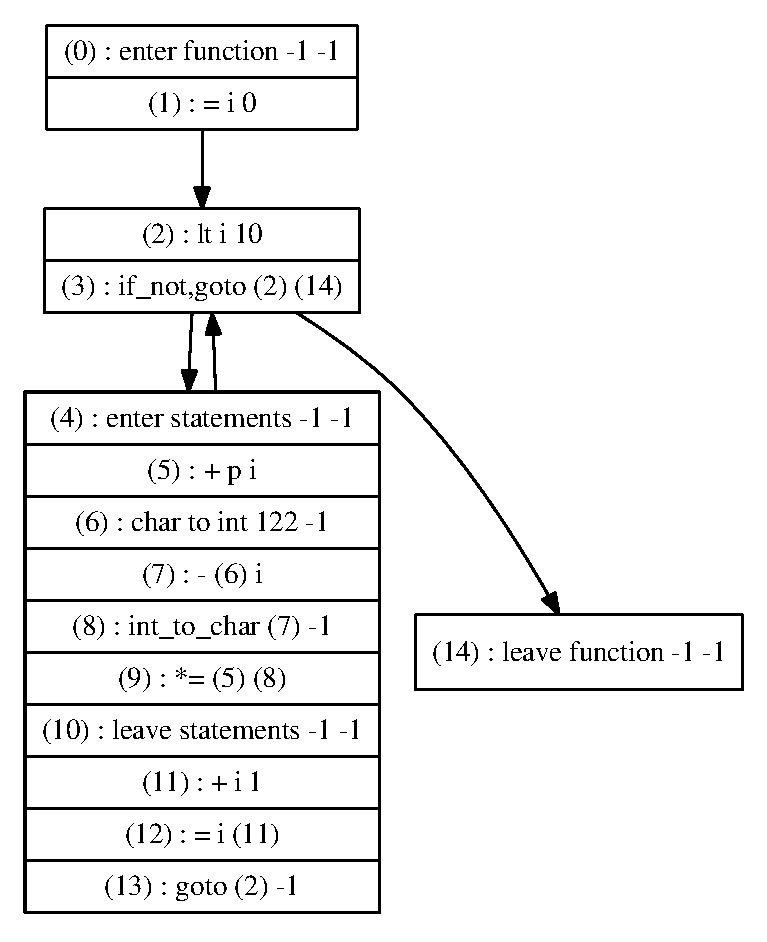
\includegraphics[scale=0.5]{basic_block}
	\captionof{figure}{基本块示例}
\end{center}
{\it \manerrarrow MiniC的验证工具中提供了生成基本块图形表示的dot文件的方法,请参阅MiniC使用手册}\\
\section{机器无关优化}
\label{indepopt}
%TODO:
MiniC在三元式表示上进行了如下优化:
\begin{itemize}
	\item 窥孔优化:常量表达式计算和面向机器的强度削减
	\item 基于数据流分析的可用表达式传播和指针分析
\end{itemize}
另外,活跃变量分析虽然不能算是优化的一部分,但由于也是基于数据流分析的迭代模型的算法,因此也在本节介绍。

\subsection{窥孔优化}
\label{peephole:intermidiate}
我们首先对三元式进行了简单的窥孔优化:
\subsubsection{常量表达式计算} 对于操作数都是常量的三元式,我们计算出该三元式的值,如果用到该三元式值的三元式又能够直接计算,那么要迭代地进行这个过程,直到结果是编译时不可计算的为止。由于目标代码生成方面的需要,这个优化不考虑对于带有常数的布尔运算。
\paragraph*{算法}

\paragraph*{示例}
下面左图是优化前的一段三元式,右图是优化后的结果:
\begin{center}
\begin{minipage}{0.4\textwidth}
\begin{center}
	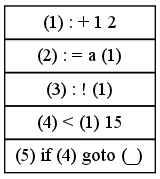
\includegraphics[scale=0.50]{before_const_expr.png}
	\label{fig:beforconstexpr}
\end{center}
\end{minipage}
\begin{minipage}{0.4\textwidth}
\begin{center}
	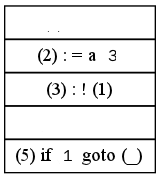
\includegraphics[scale=0.50]{after_const_expr.png}
	\label{fig:afterconstexpr}
\end{center}
\end{minipage}
\captionof{figure}{常量表达式优化示例}
\end{center}
\paragraph*{简单的强度削减} 虽然这部分是机器相关的(在Unicore32中,乘法指令需要2 CPU cycles,而移位指令仅需要1 CPU cycle),但在三元式部分做较为简单,即把乘以2的幂次的三元式都替换成左移幂次位数的三元式。在目标代码生成阶段,左移的三元式会被翻译成移位\verb|mov|,然后通过目标代码的窥孔优化将其和其它代码合并。

\subsection{数据流分析及相关优化}
\label{dataflow}
数据流分析技术都基于相似的算法框架和数据结构,只是在初值和迭代方程处不同。下面将介绍我们用于数据流分析的数据结构,并将重点介绍我们设计或改造的数据流分析算法。

数据流分析算法的范围是一个函数,因此下面的讨论的都是怎样在单个函数中进行数据流分析。

\subsubsection{基础数据结构}
\label{jointtable}
数据流分析算法具有以下特点:
\begin{itemize}
	\item 每一个“程序点”,即每个三元式之前和之后,都有不同的状态集,并且该状态集的成员可能是所有三元式(标号,也即临时变量)或所有变量
	\item 状态集成员的状态只有2种
	\item 需要多次迭代,每个基本块的输入或输出是根据其前驱的输入和输出进行交汇运算而得,交汇运算一般为集合并或集合交,因此需要能够快速进行这两种操作的集合表示。 
\end{itemize}
这些特点决定了数据流分析算法需要位向量来表示状态集,因此就会引出如何将变量或或三元式标号映射到位向量的某一位的方法;与此同时,一些算法还需要快速判断两个变量名是否代表同一个变量(因为有不同的作用域),所以我们为每一个有值的三元式建立了符号表项,并使用了一个“联合查询表”统一地保存函数中出现的所有变量和标号的符号表项指针。我们还将三元式中操作数及结果所代表的变量或标号在“联合查询表”中的位置保存了在三元式的结构中。现在,某个变量或标号在位向量中的位置就是它在“联合查询表”中的索引;比较变量相同只需判断它们在“联合查询表”中的索引是否相等。

由于是在函数范围内做数据流分析,因此我们还建立了表示一个函数的数据结构,它包含了指向该函数首、尾基本块的指针以及该函数的所有数据流分析状态信息,还包括了以后的寄存器分配信息。
\begin{lstlisting}
typedef struct func_block {
	basic_block* start; //函数入口基本块
	basic_block* over; //结束基本块
	struct func_block* prev; //函数链中上一个函数
	struct func_block* next; //函数链中下一个函数

	int code_num; //函数中三元式个数
	int bb_num; //函数中基本块个数
	symtbl_item** uni_table; //“联合查询表”
	int uni_item_num;
	int uni_table_size;
	
	map_table* mapping; //记录“联合查询表”中标号的映射信息
	int map_table_size;	
	/*活跃变量分析信息*/
	... 
	/*----------------*/
	
	/*可用表达式分析信息*/
	...
	/*------------------*/
	
	/*寄存器分配信息*/
	...
	/*------------------*/

}func_block;
\end{lstlisting}
{\it \anchor 有关\verb|func_block|的完整定义以及“联合查询表”的建立方法,请参阅:\verb|basic_block.h|, \verb|prepare_dataflow.c|}\\

活跃变量分析和可用表达式分析算法参见\cite{sunjiasu}中第9章。下面介绍两个我们改进和设计的关于数据流分析的优化算法。
\subsubsection{可用表达式传播}
这种算法只利用可用表达式信息,产生的效果类似于但劣于复写传播。

\paragraph*{目的}某些表达式在同一函数中计算了多次,需要在保证正确的情况下用第一次计算的结果代替其余计算的结果。举例如下:

在下面左图的流图中,(1)(4)(7)(9)均是相同的表达式,并且从(1)开始,a和b都没有重新定值,因此可以用(1)去替换下面出现的三元式操作数(4)(7)(9),并且删去重复计算的后三句,得到下面右图。
\begin{center}
\begin{minipage}{0.4\textwidth}
\begin{center}
	\includegraphics[scale=0.50]{before_available_expr.jpeg}
\end{center}
\end{minipage}
\begin{minipage}{0.4\textwidth}
\begin{center}
	\includegraphics[scale=0.50]{after_available_expr.jpeg}
\end{center}
\end{minipage}
\captionof{figure}{可用表达式传播示例}
\end{center}

\paragraph*{算法}
\begin{enumerate}
	\item 进行可用表达式分析
	\item 遍历三元式列表,对于一个未被修改或删除的三元式,如果它之前的程序点上有和它进行相同计算的可用表达式,那么沿着该三元式的所有非环前驱路径向上查找它所有最远的与它进行相同计算的可用表达式,如果仅找到1个,假设其标号为$i$,那么进行3,否则继续遍历三元式列表,遍历完毕则进行4。
	\item 从当前三元式向下查找所有用当前三元式标号当操作数的三元式,将该操作数替换成$i$,删除当前三元式,记录被修改的三元式,继续遍历。
	\item 如果没有三元式被删除,那么算法结束,否则进行1
\end{enumerate}
之所以进行迭代,是因为在修改三元式后,会出现新的替换机会。
\paragraph*{缺陷}
若某个三元式所计算的表达式在该点可用,但这些可用表达式没有公共的可用表达式前驱,则这种算法不能省去该三元式。例如,如果去掉上图中的(1)句,虽然插入赋值语句后再运用复写传播仍然能够将(9)省掉,但由于本算法的只进行简单的替换而不进行语句的插入,所以不能确定应当将(9)替换成(4)还是(7)。这个缺陷的更深层次的原因请见本章的\hyperref[pitfallc2]{“谬误与陷阱”}。\\

{\it \anchor 有关可用表达式传播的代码,请参阅:\verb|available_expr.c|}\\
\subsubsection{指针分析}
在面向RISC结构的处理器的C编译器实现中,为了提高运算性能,大部分的变量留在寄存器中以减少访存次数。但是指针能够直接访问变量所属的内存位置。因此,需要保证在指针操作后,某个变量在寄存器中的值和其在栈帧中的值同步,为了掌握需要将哪些变量在内存中的值更新这一信息,我们需要对三元式代码进行指针分析。
为此,我们设计了一个基于数据流分析的算法,来相对精确地得到在某一点每个指针可能指向哪些变量。
\paragraph*{算法}基于数据流分析迭代框架:
\begin{itemize}
\item 操作集合是指针-变量序对\verb|(p,v)|的集合
\item 对于每个基本块$B$,$GEN(B)$是在该块中产生的指针-变量序对(即有指针赋值或取地址操作),$KILL(B)$是在该块中注销的指针-变量序对(如果某指针指向了别的变量,就注销掉该指针以前指向的变量)
\item 迭代顺序:正向;迭代方程:$OUT(N) = GEN(N)+(IN(N)-KILL(N))$\\$IN(N)=\bigcup_{P\in predecessor(N)}OUT(P)$
\end{itemize}
\paragraph*{性能}
我们将结合一个例子来比较以下三种算法:
\begin{itemize}
	\item 假设某个指针可能指向所有变量,即遇到指针访问就同步所有的变量
	\item 扫描一遍代码,记录某个指针可能指向哪些变量,只同步可能指向的变量
	\item 基于数据流分析的指针分析
\end{itemize}
\begin{lstlisting}
int f()
{
	int a,b,c,*p,*q;
	...
	if(some_condition)
		p = &a;
	else
		p = &b;
	*p = 1;
	while(some_condition){
		q = p;
		*q = 1;
		q = &c;
		*q = 2;
	}
	...

}
\end{lstlisting}
第一种算法将在第9行、第12行和第14行将\verb|a, b, c|全部同步;第二种算法在第9行同步\verb|a, b|,在第12行和第14行同步\verb|a, b, c|;第三种算法将在第12行同步\verb|a, b|,在第12行同步\verb|a, b, c|,在第14行同步\verb|c|。

可以看出,基于数据流分析的指针分析具有更好的精确性,因此能够节省更多的内存操作的次数。\\
{\it \anchor 有关指针分析的代码,请参阅:\verb|pointer_analysis.c|}\\

\subsubsection{一些对数据流分析的改进设想}
\paragraph*{全局指针分析}
当前MiniC的指针分析算法只能得到函数内的指针可能指向的变量,但是将指针作为参数传入另一个函数后,由于得不到该指针可能指向的地址,只能在调用函数时保存所有局部变量。如果能将指针分析的范围扩大到整个源文件,那么就能够得到完整的指向信息,从而彻底地解决正确、节约地同步寄存器和内存的问题。
\paragraph*{全局活跃变量分析}
当前MiniC的活跃变量分析算法只能得到函数内的活跃变量信息。改进的可能同样来自函数调用:如果能够得到被调用的函数将占用哪些寄存器,就能够在调用前只保护这些寄存器,从而节省一些访存语句。这有赖于全局的(跨函数的)活跃变量分析。
\section{谬误与陷阱}
\label{pitfallc2}
\subsection*{中间表示设计的小缺陷将会引起许多不便}
\paragraph*{AST的修剪}
MiniC建立的AST没有经过任何修剪,从图\ref{fig:grammertree}的示例中可以看出,一些无用的语法符号(例如括号、逗号)仍然留在AST上,并且在声明和语句等子树上存在着大量的左递归子树。

在设计之初,我们忽略了这些多余的节点和复杂的左递归结构可能带来的问题。但当使用这棵AST生成了符号表并且进行了类型检查后,我们发现如果事先对AST进行一些简单的预处理,消除掉冗余的部分,替换掉复杂的结构,就能够避免使用AST时复杂的条件分支,也能够避免因为复杂的结构而造成的代码逻辑上的错误。

\paragraph*{三元式,四元式}
在设计之初,我们认为三元式和四元式在表达能力上是等价的,并且发现三元式有良好的结构使得在其上构建DAG更方便,于是MiniC采用了三元式作为第二重中间表示。

然而,三元式的特点也是它的缺点:因为标号同时也代表临时变量,因此在三元式表示中,临时变量只能赋值一次。这个缺陷影响了后面的两部分工作:
\begin{itemize}
\item 在翻译布尔表达式时,必须允许某个标志变量被赋值两次,否则布尔表达式的赋值(如\verb|a=b&&c|)将无法实现。因此我们向三元式中添加了\verb|setrb|和\verb|getrb|两条语句。虽然在目标代码生成阶段没有直接翻译这两条语句,而是转换成了效率更高,更易读的汇编代码,这种表示仍然给我们带来了不少麻烦。
\item 在进行基于三元式的优化时,由于发现了可用表达式但无法在多处插入给同一个临时变量赋值的三元式(见\cite{sunjiasu}第216页),我们只好放弃性能更为强大的可用表达式-复写传播来消除冗余中间代码,改为使用可用表达式传播的算法。
\end{itemize}

\chapter{目标代码}
\label{targetcode}
在对源文件进行了足够的检查、变换并且提取了足够的信息后,应当具备了以下条件:
\begin{itemize}
	\item 确保源文件语法、语义正确
	\item 有一个同目标汇编码接近的中间表示
	\item 有一个能够查询标识符(包括源文件中的符号和中间表示中的临时变量)信息的接口
\end{itemize}
接下来就可以开始生成目标代码了,我们将在这一章介绍编译器观点下的作为目标机器的Unicore32体系结构、MiniC将三元式表示翻译成Unicore32汇编语言的过程以及MiniC在目标代码上进行的机器相关优化。
\section{编译器-目标机器二进制接口}
\label{target_machine}
本节介绍编译器视角下的Unicore32体系结构,主要包括寄存器使用情况和内存的维护(包括栈帧和全局区)。

{\it \anchor 有关Unicore32指令系统,请参阅:《Unicore32处理器ISA(子集)介绍》}\\

\subsection{寄存器使用情况}
下表对照了UniCore32的寄存器使用规范和MiniC的寄存器使用情况:
\begin{center}
	\begin{tabular}{|l|l|l|}
	\hline
		寄存器 & Unicore32寄存器使用规范 & MiniC \\
	\hline
		r0-r3 & 传递参数;r0保存返回值 & 传递参数;r0保存返回值;在函数内用于无寄存器变量的装入和运算 \\
	\hline
		r4-r15 & caller save & caller save,个数可调$^*$\\
	\hline
		r17-r25 & callee save & callee save,个数可调$^*$\\
	\hline
		r26 & 静态基址 & 装入全局变量地址\\
	\hline
		r27 & 栈帧基址 & 栈帧基址\\
	\hline  
		r28 & 调用者SP & 传参时用于装入和运算(由于此时r0-r3不能用于运算);生成立即数\\
	\hline 
		r29 & 栈基址 & 栈基址 \\
	\hline
		r30 & 返回地址 & 返回地址 \\
	\hline 
		r31 & PC & PC \\
	\hline
	\end{tabular}
	\label{registerstat}
\end{center}
{\it $^*$\verb|register_stat.h|用于调整可用的caller save和callee save寄存器的个数}

注意到r28的用法和规范有差异,但这不影响MiniC生成的目标文件同其它Unicore32编译器生成的目标文件的链接。
\subsection{内存的维护}
\subsubsection{栈帧的维护}
在程序运行之初,装载器给r29赋初值后,维护栈帧的工作交由程序自己来进行。因此编译器需要在目标代码中添加相关代码。

栈帧维护的汇编语句将在翻译表示函数调用的三元式(\verb|param|和\verb|call|)时产生。

下图左图展示了函数调用时栈帧的情况,右图展示了局部数组的保存方法:
\begin{center}

\begin{minipage}{0.4\textwidth}
\begin{center}
	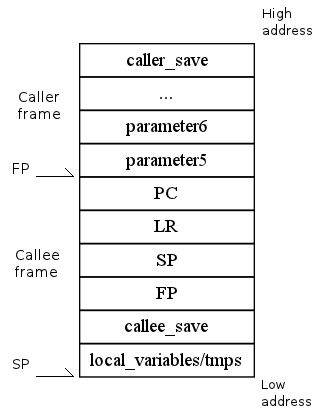
\includegraphics[scale=0.6]{stack_frame.png}
	\label{fig:stackframe}
\end{center}
\end{minipage}
\begin{minipage}{0.4\textwidth}
\begin{center}
	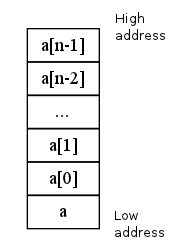
\includegraphics[scale=0.6]{local_array.png}
	\label{fig:localarray}
\end{center}
\end{minipage}
\captionof{figure}{栈帧与局部数组示意图}
\end{center}
FP以上(高地址方向)是调用者的部分栈帧(略去部分和被调用者栈帧相似),其中保存了call save寄存器以及传给被调用者的从第5个到最后一个参数(如果被调用者参数小于等于4,那么省去这一段)。

FP到SP的一段是被调用者的栈帧,其中保存了调用时的PC,返回地址,调用者的栈顶地址和栈帧基址以及callee save寄存器的值。同时,每一个局部变量和没有分配寄存器的临时变量在栈帧中均有位置。

对于局部数组,数组的头指针存放在数组起始的第一个字节,即不考虑对齐的情况下一个$4n$字节的\lstinline|int|数组将占用$4n+1$的空间。

\subsubsection{全局区的维护以及大立即数的处理}
我们将全局变量(或数组)、字符串常量保存在全局区中。由于全局区可能较大,使用基址和偏移量的寻址方式很可能出现偏移量过大不能使用带立即数的访存指令的问题。为此,我们将每个函数需要用到的全局变量的指针保存在该函数的代码段末尾,并分配给它们一个标号。当使用这些标号寻址时,汇编器会自动将寻址方式转换成PC相对寻址。

对于无法使用立即数寻址的三元式中的立即数,我们也将它保存在函数的代码段末尾,通过PC相对寻址将其读入。

例如下述代码:
\begin{lstlisting}
int a,b;
int f()
{
	a=25500;
	b=25500;
}

\end{lstlisting}
我们将生成如下的汇编代码:
\begin{verbatim}
	.comm	b, 4, 4
	.comm	a, 4, 4
	.text
	.global	main
	.type	main,function
main:
	@Create stack frame
.L1:
	ldw	r3, .L3+8
	ldw	r1, .L3+0
	stw	r3, [r1+], #0
	ldw	r3, .L3+8
	ldw	r1, .L3+4
	stw	r3, [r1+], #0
	@End of program
.L3:
	.word	a
	.word	b
	.word	25500
\end{verbatim}
\section{寄存器分配}
\label{registeralloc}
Unicore32采用RISC结构,具有31个通用寄存器,所以对于大部分程序,几乎所有变量都可以保存在这些寄存器中,以减少对内存的读写。因此需要一个方法来给每个变量关联一个寄存器,该方法需要保证能用最节约的方式分配,同时变量之间不能互相污染。

MiniC采用了启发式的图染色寄存器分配算法。该算法依赖于在三元式上进行的活跃变量分析的结果,即需要在某个程序点上每个变量的活跃信息,然后建立一个干涉图$G(V,E)$,其中$V$是变量的集合,$(v_1,v_2)\in E$当且仅当存在某个程序点,使得在此处$v_1$和$v_2$同时活跃。给变量分配寄存器就相当于给这张干涉图着色。

举例如下,对于左图的三元式序列(花括号中是该句处的活跃变量),干涉图为右图:
\begin{center}

\begin{minipage}{0.4\textwidth}
\begin{center}
	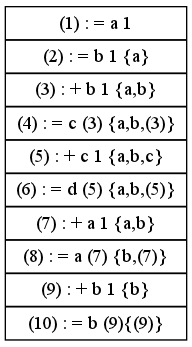
\includegraphics[scale=0.6]{register_allocation_triple.png}
	\label{fig:registerallocationtriple}
\end{center}
\end{minipage}
\begin{minipage}{0.4\textwidth}
\begin{center}
	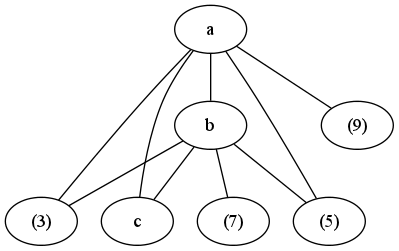
\includegraphics[scale=0.6]{interference_graph.png}
	\label{fig:interferencegraph}
\end{center}
\end{minipage}
\captionof{figure}{寄存器分配示例}
\end{center}
下表给出了不同的可分配寄存器数目的寄存器分配的结果:
\begin{center}
	\begin{tabular}{|l|l|l|}
	\hline
		变量 & 2个可用寄存器 & $\geq$3个可用寄存器 \\
	\hline
		a & 保存在内存 & r6 \\
		b & r5 & r5 \\
		c & r4 & r4 \\
		(3) & r4 & r4 \\
		(5) & r4 & r4 \\
		(7) & r4 & r4 \\
		(9) & r4 & r4 \\
	\hline
	\end{tabular}
	\captionof{table}{寄存器分配示例}
\end{center}
注意到在只有2个可用寄存器时,出现了寄存器不足的情况。对于这种情况MiniC会选择将某些变量保存在内存(即在干涉图中删除该顶点)。这些保存在内存的变量每次引用都需要读取内存;每次赋值都需要写入内存。在\cite{sunjiasu}中介绍的算法采用的选择策略是总选择度数最大的点删除,但是在一些对数组频繁操作的程序实例(如排序算法)中,采用这种策略将会使得数组基址被保存在内存中,使得每次读取数组元素之前要先读取基址,大大影响了性能。我们认为可以采用一种更为折衷的办法:综合考虑变量的使用频率和它的干涉边数,给出一个权衡后的解。但由于时间关系,这一想法没有实现。\\
{\it \anchor 有关寄存器分配和活跃变量分析的代码,请参阅:\verb|register_allocation.c|, \verb|live_var_anal.c|}\\
%TODO:三元式转换为目标代码
\section{将三元式转换为目标代码}
\label{tripletotarget}
\subsection{控制流语句的翻译}

\subsection{寄存器保护与同步}
\label{registerprotect}
\subsection{立即数的处理}

{\it \anchor 有关三元式转换为目标汇编码的代码,请参阅:\verb|gen_target_code.c|}\\
\section{机器相关优化}
\label{depopt}
在生成目标代码的过程中,我们已经对一些潜在的代码冗余进行了清理,但是受到中间表示和翻译方法的限制,生成出的目标代码仍有改进的余地,下面介绍我们在目标代码上,配合Unicore32指令系统进行的优化。
\subsection{窥孔优化}
\label{peephole:target}
{\it \anchor 有关目标代码上的窥孔优化的代码,请参阅:\verb|peephole.c|}\\
\subsubsection{合并访存语句}
如\verb|a[i] = 1|这样的MiniC语句翻译成的三元式如下:
\begin{center}
	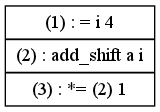
\includegraphics[scale=0.50]{merge_ldst.png}
	\captionof{figure}{合并访存语句示例}
	\label{fig:mergeldst}
\end{center}
根据三元式生成的目标代码为(假设r4中保存着a的基址,r5中保存着i的值):
\begin{verbatim}
add r5, r4, r5<<#2
mov r3, #1
stw r3, [r5+], #0
\end{verbatim}
由于Unicore32提供了“寄存器位移读取(写入)”的指令,这个操作事实上只需要:
\begin{verbatim}
mov r3, #1
stw r3, [r4+],r5<<#2
\end{verbatim}
由于\verb|add|和\verb|stw|可能不连续,逐句生成目标代码时,发现合并的可能较为困难,因此我们扫描生成出的代码,将所有符合上面例子中的情况都进行了合并。

这项简单的优化在循环地对数组访问的情况下对性能的提升比较明显。
\subsubsection{消除冗余的\lstinline|mov|}
由于三元式的一些局限,翻译得到的目标代码在读取内存操作的附近可能会有一些冗余的\verb|mov|语句,本优化类似于复写传播,目的是将这些\verb|mov|删除。

能被删除的\verb|mov|具有以下条件:
\begin{itemize}
	\item 从mov指令的源操作数最近的一次定值开始,到mov指令之间没有对mov的目标操作数引用。
	\item 从mov指令开始,将mov指令的源操作数替换为目标操作数时不会产生冲突。
\end{itemize}
\paragraph*{算法}
\begin{enumerate}
\item 对目标代码划分基本块(以跳转指令为标志),并在基本块上做一个简单的跳转关系图,每个基本块中记录每个它接下来可能执行的基本块。
\item 扫描代码。对每个mov语句,其目标寄存器为$Rd_{mov}$,源寄存器为$Rm_{mov}$。从该条语句向上寻找最近一条语句i,语句i的目标寄存器为$Rm_{mov}$。(语句$i$对$Rm_{mov}$定值)
\item 判断语句$i$是否可以被删除。原则有:
	\begin{itemize}
		\item 若$mov$语句到语句i之间有对$Rd_{mov}$的引用,则不可删除。
		\item 从语句$i$开始,根据跳转关系图向后扫描代码(深度优先的遍历)。若进入循环块则停止,语句$i$不可删除。
		\item 扫描过程中,若某调语句引用了$Rm_{mov}$,则将它替换为$Rd_{mov}$。若某条语句对$Rm_{mov}$定值,则这条扫描路径终止。若某条语句对$Rd_{mov}$定值,并在这之后又引用$Rm_{mov}$,则扫描停止,语句$i$不可删除。
	\end{itemize}
\item 若上述扫描完成后,没有出现语句$i$不可删除的情况,则删除$mov$语句,将语句$i$的目标寄存器改为$Rd_{mov}$。
\end{enumerate}

\paragraph*{示例}
注意到在进行消除后,使用\verb|r4|作为源寄存器的\verb|add|语句改为使用\verb|r5|。
\begin{center}
\includegraphics[scale= 0.6]{redundent_mov_remove.png}
\end{center}

\subsection{尾递归优化}
\label{tailrecursion}
尾递归优化能将符合下面条件的函数调用转化成迭代:
\begin{itemize}
	\item 递归调用
	\item 该调用语句是本函数除返回语句以外的最后一条语句
	\item 该函数没有返回值
\end{itemize}
例如下面的快速排序代码:
\begin{lstlisting}
void qsort(int* data, int begin, int end)
{
	int i,j,tmp;
	if(end <= begin + 1)
		return;
	/* partition routine */
	...
	qsort(data, begin, j - 1);
	qsort(data, j, end);
	return;
}
\end{lstlisting}
注意到第9句的调用符合尾递归条件,因此我们将迭代地处理本次调用:将\verb|data, j, end|分别放在分配给对应参数的寄存器中,然后无条件跳转到函数的开始部分,建立栈帧的语句之后。下面两图对比了生成的目标代码:
\begin{center}
	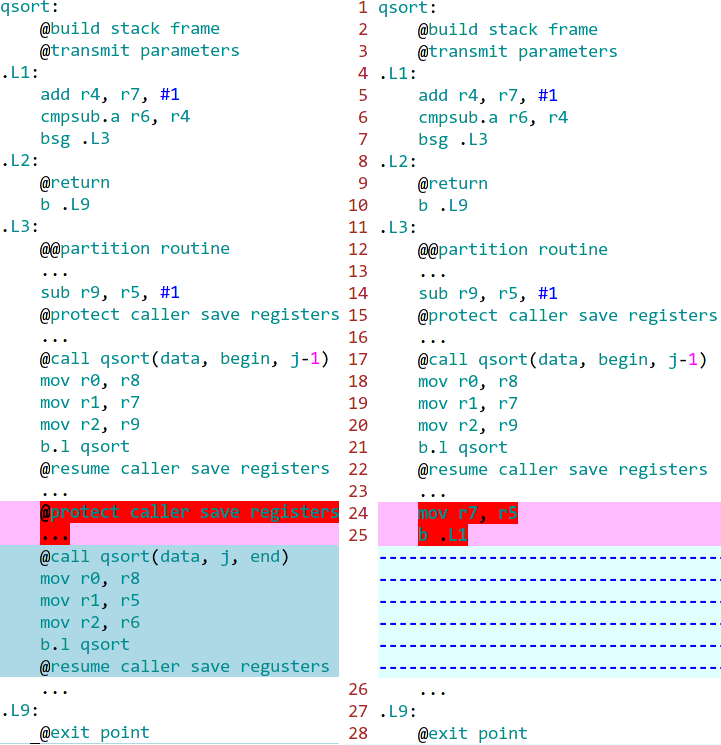
\includegraphics[scale=0.44]{tail_recursion.png}
	\captionof{figure}{尾递归示例}
	\label{fig:tailrecursion}
\end{center}
可以看出,在第二个\verb|qsort|的调用时(24行-30行),进行尾递归优化的程序(右)直接将新值\verb|j|传入被修改的参数\verb|begin|所在的寄存器\verb|r7|中,然后无条件跳转到了函数的正文标号\verb|.L1|。节省了保存、恢复现场以及新调用建立栈帧的指令。\\
\paragraph*{缺陷}
如果对一个通过传入自己局部变量指针的而修改上一栈帧局部变量内存内容的函数进行尾递归优化将产生执行结果的错误。因此MiniC默认关闭了尾递归优化,只有当程序员保证没有上述情况时可以选用开启。\\
{\it \anchor 有关尾递归优化的代码,请参阅:\verb|gen_target_code.c|}\\

\subsection{指令调度}
\label{assembledispatch}
根据Unicore32指令系统体系结构,除了载入和运算指令可能产生的数据相关无法转发,需要等待一个cycle以外,其它指令的数据相关均已通过转发解决。指令调度的目的是减少甚至消除因载入指令而造成的数据相关。

\paragraph*{算法}
\begin{enumerate}
	\item 在目标代码上划分基本块(以跳转指令和标签作为标记)。指令调度在基本块内完成。
	\item 对每个基本块,根据指令间的数据依赖关系,建立数据依赖图。若指令$i$的源操作数依赖于指令$j$的执行结果,则建立$j$到
$i$的一条边。
	\item 根据数据依赖图,进行变种的拓扑排序:扫描块中所有指令。遇到\verb|ldw|指令,则开始执行所有\verb|ldw|指令依赖的指令(即在图上可达这条\verb|ldw|指令的指令);之后,从所有本块中未执行过的指令中取出一条入度为0的指令(不依赖于任何指令),排在这条\verb|ldw|指令后面。特别地,这条指令的源操作数应该尽量和\verb|ldw|指令的目标操作数不相等。
	\item 扫描一遍\verb|ldw|指令之后,所有可能调开的\verb|ldw|指令都已经被调开。再对未执行的指令进行拓扑排序即可。
\end{enumerate}
\paragraph*{示例}
下面是一段汇编指令:
\begin{verbatim}
	ldw	r4, [r6+], #4
	add	r5, r4, r5
	ldw	r4, [r6+], #4
	sub	r4, r4, r5
	ldw	r30, [r27+], #-4
\end{verbatim}
它的依赖关系图如下:
\begin{center}
	\includegraphics[scale=0.35]{assemble_rely_graph.png}
\end{center}
调度后的指令序列:
\begin{verbatim}
	ldw	r4, [r6+], #4
	add	r5, r4, r5
	ldw	r4, [r6+], #4
	ldw	r30, [r27+], #-4
	sub	r4, r4, r5
\end{verbatim}
{\it \anchor 有关指令调度的代码,请参阅:\verb|instruction_dispatch.c|}\\
\section{谬误与陷阱}
\label{tarpitc3}
\subsection*{编译优化与结果正确性}
教科书上对编译优化的要求是:以\emph{正确}为前提,尽可能地提升目标代码的效率。然而在实践中,存在着一些对“正确”定义不清的灰色地带,如果一味地追求绝对正确,将大大损失性能。例如对如下的一段C代码:
\begin{lstlisting}
void f(int* p)
{
	*p = 1;
}
int main()
{
	int a,b,c,*p;
	p = &b;
	p += 1;
	//*p = c 
	f(p);
}
\end{lstlisting}
按照原则上来说,如果一个程序员对他所面对的目标机器足够了解的话,\verb|p += 1|的使用也许是为了指向\verb|a|(或\verb|c|),因此在调用函数\verb|f|的时候应当将\verb|a|(或\verb|c|)的值同步到内存中以保证“正确”。

然而\verb|unicore32-linux-gcc|使用\verb|-O2|编译参数的结果却是错误的:它没有做任何的访存操作来保护内存和寄存器的同步。

原因是\verb|gcc|在性能和“绝对正确”之间做出了权衡:应该由程序员而不是编译器应该保证这种极为特殊的情况的正确性。

这样做所换来的性能提升也是可观的:在不考虑指针计算的情况下,简单的数据流指针分析就能够精确地得到应该同步的变量。

为了在绝大部分情况下提高性能,MiniC也要求这种特殊情况由程序员自行保证。(去掉上面代码中的注释即可)

当然,在“保证绝对正确”的编译选项下,情况又不同了,这时候就算牺牲性能也要保证没有任何差错。



\chapter{编译-体系联合实验}

本章介绍了编译实习-体系实习联合项目中进行的实验。在实验中,我们控制和调整了如下参数:
\begin{itemize}
	\item 可用的通用寄存器数目
	\item 是否进行指令调度
\end{itemize}
我们使用了两个评测程序:快速排序和矩阵乘法。

\input{appendix}
\begin{thebibliography}{99}
\bibitem{sunjiasu}孙家骕,编译原理,北京大学出版社,2008
\end{thebibliography}
\end{document}
